\begin{pr}$ $
\begin{enumerate}[(a)]
\item Recall that the CDF of $\mathrm{Exponential}(\lambda)$ is $1-e^{-\lambda x}$, and its mean is $\frac1\lambda$.\\
False alarm probability $=\P[T>t_0|H_0]=\P[T>t_0|T\sim\mathrm{Exponential}(\frac13)]=1-\P[T\leq t_0|T\sim\mathrm{Exponential}(\frac13)]=1-1+e^{-\frac{t_0}3}=e^{-\frac{t_0}3}$.
\item Miss probability $=\P[T\leq t_0|H_1]=\P[T\leq t_0|T\sim\mathrm{Exponential}(\frac1{\mu_O})]=1-e^{-\frac{t_0}{\mu_O}}$.
\item We want $t\leq t_0\iff f_{T|H_0}(t)\geq f_{T|H_1}(t)$.\\
Recall that the PDF of $\mathrm{Exponential}(\lambda)$ is $\lambda e^{-\lambda x}$.\\
$\so$ we want $t\leq t_{ML}\iff\frac1{\mu_O}e^{-\frac t{\mu_O}}\leq\frac13e^{-\frac t3}$.\\
$\frac1{\mu_O}e^{-\frac t{\mu_O}}\leq\frac13e^{-\frac t3}\iff\frac3{\mu_O}\leq e^{t(\frac1{\mu_O}-\frac13)}\iff\ln\frac3{\mu_O}\leq t(\frac1{\mu_O}-\frac13)\overset{\cuz\mu_O>3}\iff t\leq\frac{\ln\frac3{\mu_O}}{\frac1{\mu_O}-\frac13}$.\\
$\so t_{ML}=\frac{\ln\frac3{\mu_O}}{\frac1{\mu_O}-\frac13}$.\\
For $\mu_O=6$, $t_{ML}=\frac{\ln\frac12}{-\frac16}=6\ln2$.\\
For $\mu_O=10$, $t_{ML}=\frac{\ln\frac3{10}}{-\frac7{30}}=\frac{30}7\ln\frac{10}3$.
\item $t_{MAP}$ is such that $t=t_{MAP}$ minimizes $f(t):=0.8\P[T>t|H_0]+0.2\P[T\leq t|H_1]$.\\
$\then f'(t)=\frac{d(0.8-0.8\P[T\leq t|H_0]+0.2\P[T\leq t|H_1])}{dt}=-0.8f_{T|H_0}(t)+0.2f_{T|H_1}(t)=0$.\\
$\then f_{T|H_1}(t)=4f_{T|H_0}(t)$.\\
Since $g(t):=\frac{f_{T|H_1}(t)}{f_{T|H_0}(t)}=\frac{\mu_O}3e^{(\frac1{\mu_O}-\frac13)t}$ is a decreasing function of $t$ ($\cuz\frac1{\mu_O}-\frac13<0$), there is $t_{MAP}=g^{-1}(\frac14)>g^{-1}(1)=t_{ML}$.
\item As in (d), $f_{T|H_1}(t)=4f_{T|H_0}(t)$.\\
$\then\frac{\mu_O}3e^{(\frac1{\mu_O}-\frac13)t_{MAP}}=\frac14$.\\
$\then(\frac1{\mu_O}-\frac13)t_{MAP}=\ln\frac3{4\mu_O}$.\\
$\then t_{MAP}=\frac{\ln\frac3{4\mu_O}}{\frac1{\mu_O}-\frac13}$.\\
For $\mu_O=6$, $t_{MAP}=\frac{\ln\frac18}{-\frac16}=6\ln8=18\ln2$.\\
For $\mu_O=10$, $t_{MAP}=\frac{\ln\frac3{40}}{-\frac7{30}}=\frac{30}7\ln\frac{40}3$.
\item$ $\\
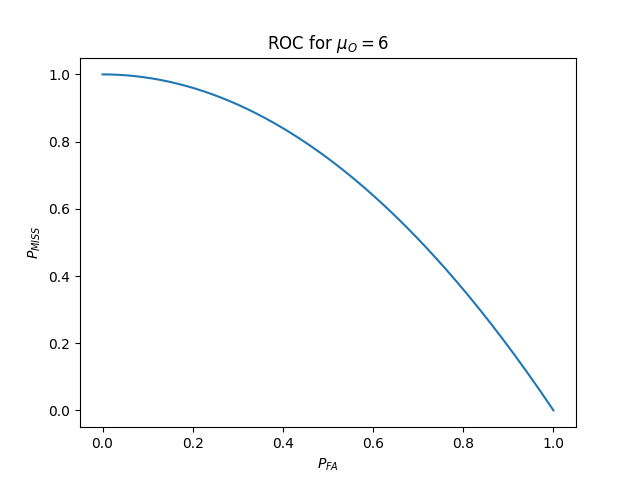
\includegraphics[width=7cm]{muO6.png}
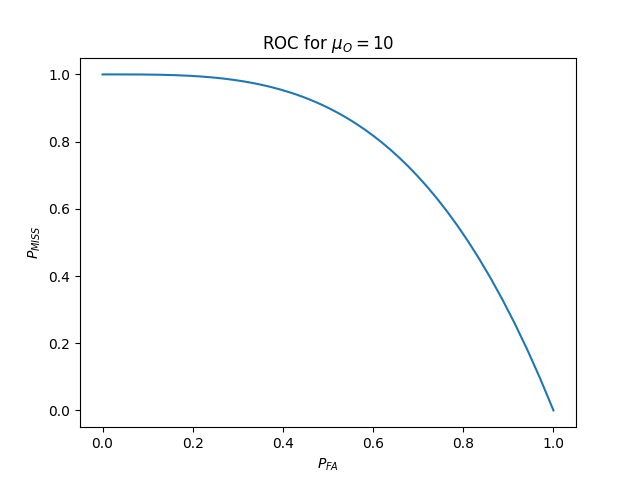
\includegraphics[width=7cm]{muO10.png}\\
I use the following code to draw the curve:
\lstinputlisting[language=python]{p1.py}
\end{enumerate}
\end{pr}
